\let\negmedspace\undefined
\let\negthickspace\undefined
\documentclass[journal]{IEEEtran}
\usepackage[a5paper, margin=10mm, onecolumn]{geometry}
%\usepackage{lmodern} % Ensure lmodern is loaded for pdflatex
\usepackage{tfrupee} % Include tfrupee package

\setlength{\headheight}{1cm} % Set the height of the header box
\setlength{\headsep}{0mm}     % Set the distance between the header box and the top of the text

\usepackage{gvv-book}
\usepackage{gvv}
\usepackage{cite}
\usepackage{amsmath,amssymb,amsfonts,amsthm}
\usepackage{algorithmic}
\usepackage{graphicx}
\usepackage{textcomp}
\usepackage{xcolor}
\usepackage{txfonts}
\usepackage{listings}
\usepackage{enumitem}
\usepackage{mathtools}
\usepackage{gensymb}
\usepackage{comment}
\usepackage[breaklinks=true]{hyperref}
\usepackage{tkz-euclide} 
\usepackage{listings}
% \usepackage{gvv}                                        
\def\inputGnumericTable{}                                 
\usepackage[latin1]{inputenc}                                
\usepackage{color}                                            
\usepackage{array}                                            
\usepackage{longtable}                                       
\usepackage{calc}                                             
\usepackage{multirow}                                         
\usepackage{hhline}                                           
\usepackage{ifthen}                                           
\usepackage{lscape}
\usepackage{multicol}
\begin{document}

\bibliographystyle{IEEEtran}
\vspace{3cm}

\title{7.4.19}
\author{EE25BTECH11012-BEERAM MADHURI}
% \maketitle
% \newpage
% \bigskip
{\let\newpage\relax\maketitle}

\renewcommand{\thefigure}{\theenumi}
\renewcommand{\thetable}{\theenumi}
\setlength{\intextsep}{10pt} % Space between text and floats


\numberwithin{equation}{enumi}
\numberwithin{figure}{enumi}
\renewcommand{\thetable}{\theenumi}


\textbf{Question}:\\
Let $\mathbf{C}$ be the circle with centre $(0,0)$ and radius $3$ units. The equation of the locus of the mid points of the chords of the circle $\mathbf{C}$ that subtend an angle of $\frac{2\pi}{3}$ at its centre is

\begin{enumerate}
\begin{multicols}{4}
    \item $x^2 + y^2 = \frac{3}{2}$
    \item $x^2 + y^2 = 1$
    \item $x^2 + y^2 = \frac{27}{4}$
    \item $x^2 + y^2 = \frac{9}{4}$
\end{multicols}    
\end{enumerate}

\textbf{Solution:}\\
Given radius = $3$ units
\begin{align}
\vec{C} = \text{center} = \begin{pmatrix} 0 \\ 0 \end{pmatrix}
\end{align}

Let $\vec{A}$ and $\vec{B}$ be the end points of chord 
\begin{align}
\|\vec{A}\| = \|\vec{B}\| = 3 \\
\vec{A}^\top \vec{A} = 9 \\
\vec{B}^\top \vec{B} = 9 \\
\vec{A}^\top \vec{B} = \|\vec{A}\| \|\vec{B}\| \cos\theta = -\frac{9}{2} 
\end{align}
Let $P$ be the midpoint of chords then, 
\begin{align}
\vec{P} = \frac{\vec{A + B}}{2} \\
\|\vec{P}\| = \frac{1}{2} \|\vec{A + B}\| \\
\vec{P^\top} \vec{P} = \frac{1}{4} (\vec{A+B})^\top (\vec{A+B}) \\
\vec{P^\top} \vec{P} = \frac{1}{4} (\vec{A^\top} \vec{A} + \vec{A^\top} \vec{B} + \vec{B^\top} \vec{A} + \vec{B^\top B})\\
\end{align}
Substituting the values:
\begin{align}
\quad = \frac{1}{4} \left(9 - \frac{9}{2} - \frac{9}{2} + 9\right) = \frac{9}{4}
\end{align}
Hence, $\vec{P^\top} \vec{P}$ =${9}/{4}$\\
option {D} is correct.
\begin{figure}[H]
    \centering
    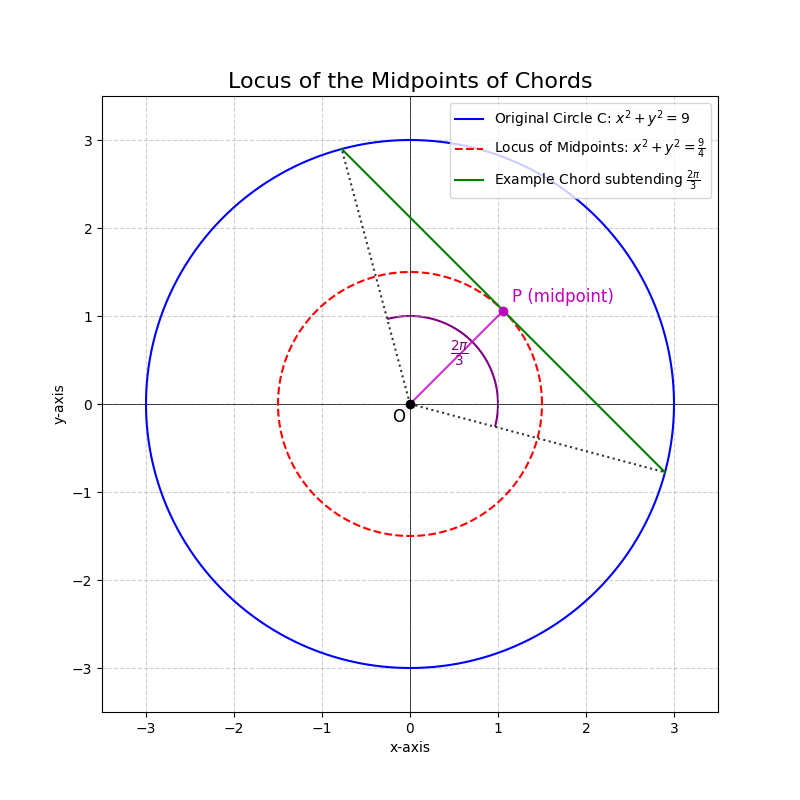
\includegraphics[width=0.85\columnwidth]{figs/graph14.png}
    \caption{7.4.19}
    \label{fig:placeholder}
\end{figure}
\end{document}
